\setchapterimage[7.5cm]{seaside}
\setchapterpreamble[u]{\margintoc}
%\chapter[Figures and Tables]{Figures and Tables\footnotemark[0]}
\chapter{Figures and Tables}

\footnotetext{The credits for the image above the chapter title go to:
	Bushra Feroz, CC~BY-SA~4.0, \url{https://commons.wikimedia.org/w/index.php?curid=68724647}}

\section{Normal Figures and Tables}

Figures and tables can be inserted just like in any standard 
\LaTeX\xspace document. The \Package{graphicx} package is already loaded 
and configured in such a way that the figure width is equal to the 
textwidth and the height is adjusted in order to maintain the original 
aspect ratio. As you may have imagined, the captions will be 
positioned\ldots well, in the margins. This is achieved with the help of 
the \Package{floatrow} package.

Here is a picture of Mona Lisa (\reffig{normalmonalisa}), as an example. 
The captions are formatted as the margin- and the side-notes; If you 
want to change something about captions you can use the command 
\Command{captsetup} from the \Package{caption} package. Remember that if 
you want to reference a figure, the label must come \emph{after} the 
caption!

\begin{figure}[hb]
	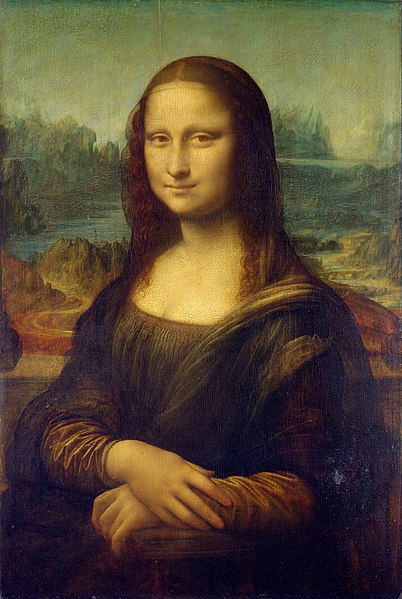
\includegraphics[width=0.45\textwidth]{monalisa}
	\caption[Mona Lisa, again]{It's Mona Lisa again. \blindtext}
	\labfig{normalmonalisa}
\end{figure}

While the format of the caption is managed by \Package{caption}, its 
position is handled by the \Package{floatrow} package. Achieving this 
result has been quite hard, but now I am pretty satisfied. In two-side 
mode, the captions are printed in the correct margin.

Tables can be inserted just as easily as figures, as exemplified by the 
following code:

\begin{lstlisting}[caption={Caption of a listing.}]
\begin{table}
\begin{tabular}{ c c c c }
	\toprule
	col1 & col2 & col3 & col 4 \\
	\midrule
	\multirow{3}{4em}{Multiple row} & cell2 & cell3 & cell4\\ &
	cell5 & cell6 & cell7 \\ &
	cell8 & cell9 & cell10 \\
	\multirow{3}{4em}{Multiple row} & cell2 & cell3 & cell4 \\ &
	cell5 & cell6 & cell7 \\ &
	cell8 & cell9 & cell10 \\
	\bottomrule
\end{tabular}
\end{table}
\end{lstlisting}

which results in the useless \vreftab{useless}.

\begin{table}[ht]
\caption[A useless table]{A useless table.}
\labtab{useless}
\begin{tabular}{ c c c c }
	\toprule
	col1 & col2 & col3 & col 4 \\
	\midrule
	\multirow{3}{4em}{Multiple row} & cell2 & cell3 & cell4\\ &
	cell5 & cell6 & cell7 \\ &
	cell8 & cell9 & cell10 \\
	\multirow{3}{4em}{Multiple row} & cell2 & cell3 & cell4 \\ &
	cell5 & cell6 & cell7 \\ &
	cell8 & cell9 & cell10 \\
	\bottomrule
\end{tabular}
\end{table}

I don't have much else to say, so I will just insert some blind text. 
\blindtext

\section{Margin Figures and Tables}

Marginfigures can be inserted with the environment 
\Environment{marginfigure}. In this case, the whole picture is confined 
to the margin and the caption is below it. \reffig{marginmonalisa} is 
obtained with something like this:

\begin{lstlisting}[caption={Another caption.}]
\begin{marginfigure}
	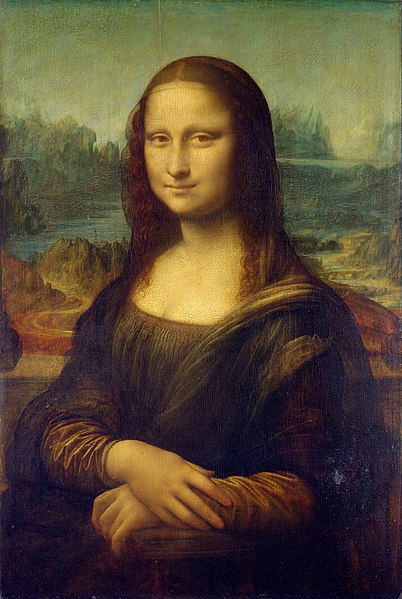
\includegraphics{monalisa}
	\caption[The Mona Lisa]{The Mona Lisa.}
	\labfig{marginmonalisa}
\end{marginfigure}
\end{lstlisting}

There is also the \Environment{margintable} environment, of which 
\reftab{anotheruseless} is an example. Notice how you can place the 
caption above the table by just placing the \Command{caption} command 
before beginning the \Environment{tabular} environment. Usually, figure 
captions are below, while table captions are above. This rule is also 
respected for normal figures and tables: the captions are always on the 
side, but for figure they are aligned to the bottom, while for tables to 
the top.

\begin{margintable}
\caption[Another useless table]{Another useless table.}
\labtab{anotheruseless}
\raggedright
\begin{tabular}{ c c c c }
	\hline
	col1 & col2 & col3 \\
	\hline
	\multirow{3}{4em}{Multiple row} & cell2 & cell3 \\ & cell5 & cell6 
	\\ & cell8 & cell9 \\ \hline
\end{tabular}
\end{margintable}

Marginfigures and tables can be positioned with an optional offset 
command, like so:

\begin{lstlisting}
\begin{marginfigure}[offset]
	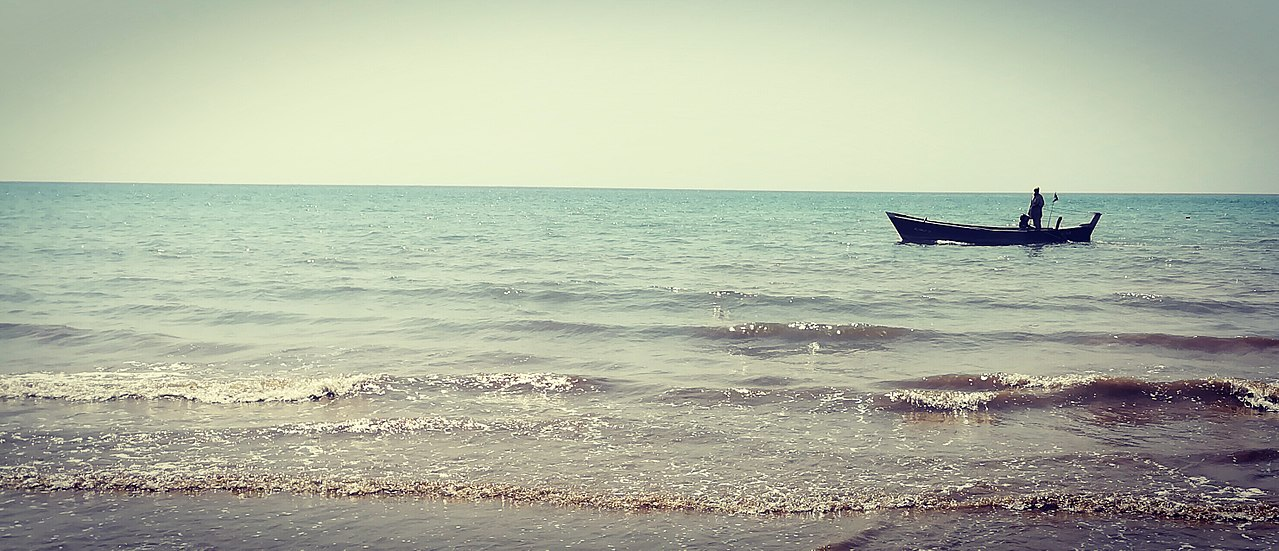
\includegraphics{seaside}
\end{marginfigure}
\end{lstlisting}

Offset ca be either a measure or a multiple of \Command{baselineskip}, 
much like with \Command{sidenote}, \Command{marginnote} and 
\Command{margintoc}.\todo{Improve this part.} If you are wondering how I 
inserted this orange bubble, have a look at the \Package{todo} package.

\section{Wide Figures and Tables}

With the environments \Environment{figure*} and \Environment{table*} you 
can insert figures which span the whole page width. For example, here 
are a wide figure and a wide table.

\begin{figure*}[h!]
	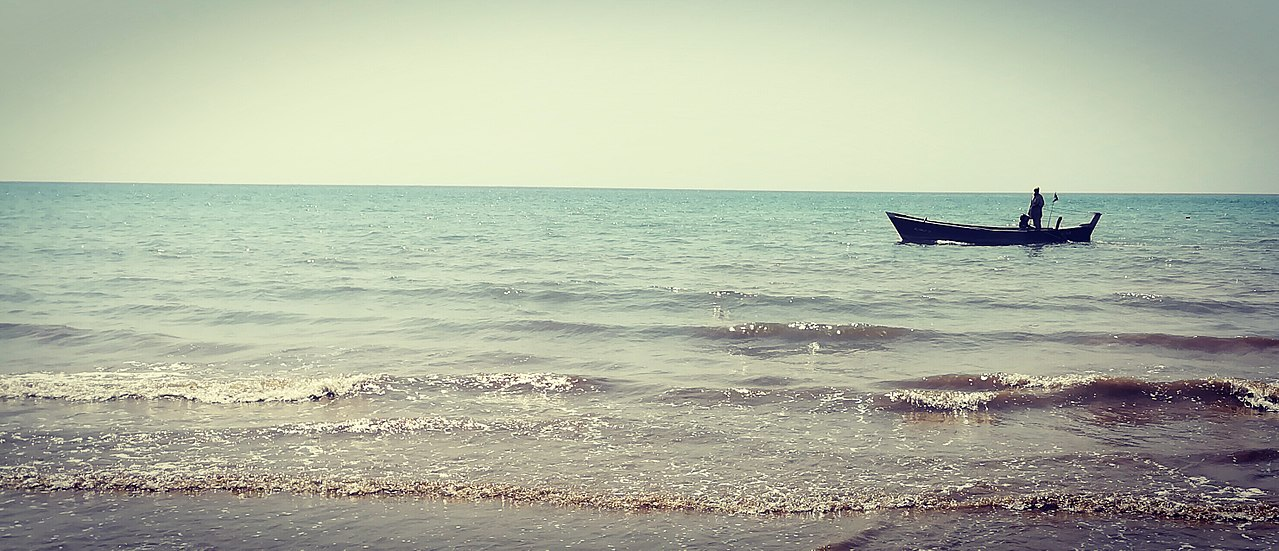
\includegraphics{seaside}
	\caption[A wide seaside]{A wide seaside, and a wide caption.
		Credits: By Bushra Feroz, CC BY-SA 4.0, \url{https://commons.wikimedia.org/w/index.php?curid=68724647}}
\end{figure*}

\begin{table*}[h!]
    \caption{A wide table with invented data about three people living in the UK. Note that wide figures and tables are centered and their caption also extends into the margin.}
    \begin{tabular}{p{2.0cm} p{2.0cm} p{2.0cm} p{2.0cm} p{2.0cm} p{2.0cm} p{1.5cm}}
        \toprule
        Name    & Surname   & Job       & Salary           & Age   & Height    & Country \\
        \midrule
        Alice   & Red       & Writer    & 4.000 \pounds    & 34    & 167 cm     & England \\
        Bob     & White     & Bartender & 2.000 \pounds    & 24    & 180 cm     & Scotland \\
        Drake   & Green     & Scientist & 4.000 \pounds    & 26    & 175 cm     & Wales \\
        \bottomrule
    \end{tabular}
\end{table*}

It is the user's responsibility to adjust the width of the table, if 
necessary, until it is aesthetically pleasing. The previous table was 
obtained with the following code:

\begin{lstlisting}[caption=How to typeset a wide table]
\begin{table*}[h!]
    \caption{A wide table with invented data about three people living in the UK. Note that wide figures and tables are centered and their caption also extends into the margin.}
    \begin{tabular}{p{2.0cm} p{2.0cm} p{2.0cm} p{2.0cm} p{2.0cm} p{2.0cm} p{1.5cm}}
        \toprule
        Name    & Surname   & Job       & Salary           & Age   & Height    & Country \\
        \midrule
        Alice   & Red       & Writer    & 4.000 \pounds    & 34    & 167 cm     & England \\
        Bob     & White     & Bartender & 2.000 \pounds    & 24    & 180 cm     & Scotland \\
        Drake   & Green     & Scientist & 4.000 \pounds    & 26    & 175 cm     & Wales \\
        \bottomrule
    \end{tabular}
\end{table*}
\end{lstlisting}

The \Package{floatrow} package provides the \enquote{H} specifier to 
instruct \LaTeX to position the figure (or table) in precisely the same 
position it occupies in the source code. However, this specifier does 
not work with wide figures or tables: you should use \enquote{h!} 
instead, like so: \lstinline|\begin{figure*}[h!]|.

You may have noticed the full width image at the very beginning of this
chapter: that, however, is set up in an entirely different way, which
you'll read about in \vrefch{layout}.

\Class{kaobook} also supports paginated tables (have a look at the 
\Package{longtable} package). The 
\Environment{longtable}\sidenote{Interestingly, \Environment{longtable}s 
may require up to four rounds of compilation before they are typeset 
correctly.} environment behaves a bit differently from 
\Environment{table}, in that \Environment{longtable} encompasses both 
\Environment{table} and \Environment{tabular}, so that you can write, 
\eg,

\begin{lstlisting}[caption=Example of a longtable]
\begin{longtable}{|l c c|}
    \hline
    One & Two & Three \\
    Left & Center & Center \\
    \hline
    \caption{Caption of the longtable.}
\end{longtable}
\end{lstlisting}

to obtain the following table:
\begin{longtable}{|l c c|}
    \hline
    One & Two & Three \\
    Left & Center & Center \\
    \hline
    \caption{Caption of the longtable.}
\end{longtable}

The caption of a \Environment{longtable} is always positioned below the 
table, and it has the same width as the text (it doesn't extend into the 
margin). However, sometimes you may need a \Environment{longtable} that 
is so wide that it trespass into the margins; in those cases, you may 
want to also increase the width of the caption. To do so, you'll have to 
write two additional commands, one before and one after the 
\Environment{longtable}:

\begin{lstlisting}[caption=Increasing the width of the caption of a \Environment{longtable}.]
\floatsetup[longtable]{margins=centering,LTcapwidth=table} % Add this line before the longtable to increase the caption width
\begin{longtable}{lp{8cm}p{5cm}p{2cm}}
...
\end{longtable}
\floatsetup[longtable]{margins=raggedright,LTcapwidth=\textwidth} % Add this line after the longtable to revert the previous change
\end{lstlisting}

Having seen figures and tables, it is now time to tackle 
hyperreferences.
